\documentclass{lab_sheet}
\usepackage{nccmath}
\usepackage{tikz}
\usetikzlibrary{arrows}
\usepackage{hyperref}
\newcommand{\figquestion}{
   \begin{circuitikz}[american]
      \draw
      (0,0) to[R,l=$1\Omega$] (4,0) to [C, *-*, l=$1.0F$] (4,-4)
      (4,0) to [L,l=$2.0H$] (8,0) to [C, *-*, l=$1.0F$] (8,-4)
      (8,0) to [short] (12,0)
      (0,0) to [esource,v_=$V_1$] (0,-4)
      (0,-4) to [short] (12,-4) to[R, l=$1\Omega$, v<=$V_2$] (12,0)
         ;
      \end{circuitikz}
}

\newcommand{\lphp}{
   \begin{circuitikz}[american]
      \draw
      (0,0) to[L,o-o,l=$L_i$] (2,0) 
      (4,0) to [C,o-o,l=$\substack{\frac{1}{\Omega_0L_i}}$] (6,0)
      (0,-2) to[C,o-o,l=$C_i$] (2,-2) 
      (4,-2) to [L,o-o,l=$\substack{\frac{1}{\Omega_0C_i}}$] (6,-2)
      ;
        \draw[->,thick](2.5,0) -- (3.5,0);
        \draw[->,thick](2.5,-2) -- (3.5,-2);
   \end{circuitikz}
}

\newcommand{\lpbp}{
   \begin{circuitikz}[american]
      \draw
      (0,0) to[L,o-o,l=$L_i$] (2,0) 
      (4,0) to [L,o-,l=$\substack{\frac{L_i}{B}}$] (6,0) to [C,-o, l=$\substack{\frac{B}{{\Omega_0}^2L_i}}$] (8,0)
      (0,-3) to[C,o-o,l=$C_i$] (2,-3) 
      (5,-2) to [L,l=$\substack{\frac{B}{{\Omega_0}^2C_i}}$] (7,-2) to [short]
      (7,-4) to [C,l_=$\substack{\frac{C_i}{B}}$] (5,-4) to [short] (5,-2)
      (5,-3) to [short,*-o] (4,-3)
      (7,-3) to [short,*-o] (8,-3)
      ;
        \draw[->,thick](2.5,0) -- (3.5,0);
        \draw[->,thick](2.5,-3) -- (3.5,-3);
   \end{circuitikz}
}

\newcommand{\lpbs}{
   \begin{circuitikz}[american]
      \draw
      (0,0) to[L,o-o,l=$L_i$] (2,0) 
      (5,1) to [L,l=$\substack{\frac{BL_i}{{\Omega_0}^2}}$] (7,1) to [short]
      (7,-1) to [C,l_=$\substack{\frac{1}{BL_i}}$] (5,-1) to [short] (5,1)
      (5,0) to [short,*-o] (4,0)
      (7,0) to [short,*-o] (8,0)
      (0,-3) to[C,o-o,l=$C_i$] (2,-3) 
      (4,-3) to [L,o-,l=$\substack{\frac{1}{BC_i}}$] (6,-3) to [C,-o, l=$\substack{\frac{BC_i}{{\Omega_0}^2}}$] (8,-3)
      ;
        \draw[->,thick](2.5,0) -- (3.5,0);
        \draw[->,thick](2.5,-3) -- (3.5,-3);
   \end{circuitikz}
}

\newcommand{\figa}{
   \begin{circuitikz}[american]
      \draw
      (0,0) to[R,l=$1.5K\Omega$] (4,0) to [C, *-*, l=$6.67nF$] (4,-4)
      (4,0) to [L,l=$30mH$] (8,0) to [C, *-*, l=$6.67nF$] (8,-4)
      (8,0) to [short] (12,0)
      (0,0) to [esource,v_=$V_1$] (0,-4)
      (0,-4) to [short] (12,-4) to[R, l=$1.5K\Omega$, v<=$V_2$] (12,0)
         ;
      \end{circuitikz}
}

\newcommand{\figb}{
   \begin{circuitikz}[american]
      \draw
      (0,0) to[R,l=$3K\Omega$] (4,0) to [L, *-*, l=$60mH$] (4,-4)
      (4,0) to [C,l=$3.33nF$] (8,0) to [L, *-*, l=$60mH$] (8,-4)
      (8,0) to [short] (12,0)
      (0,0) to [esource,v_=$V_1$] (0,-4)
      (0,-4) to [short] (12,-4) to[R, l=$3K\Omega$, v<=$V_2$] (12,0)
         ;
      \end{circuitikz}
}

\newcommand{\figc}{
   \begin{circuitikz}[american]
      \draw
      (0,0) to[R,l=$\substack{2K\Omega}$] (4,0) to [short,*-*] (4,-1)
      (4,0) to [L,l=$\substack{1H}$] (6,0) to [C,l=$\substack{0.625nF}$] (8,0) to [short, *-*] (8,-1)
      (3,-1) to [short] (5,-1) 
      (3,-1) to [L, l_=$\substack{5mH}$] (3,-3) to [short] (5,-3) to [C,l_=$\substack{0.125\mu F}$] (5,-1)
      (7,-1) to [L, l=$\substack{5mH}$] (7,-3) to [short] (9,-3) to [C,l_=$\substack{0.125\mu F}$] 
      (9,-1) to [short] (7,-1)
      (8,0) to [short] (12,0)
      (4,-3) to [short,*-*] (4,-4)
      (8,-3) to [short,*-*] (8,-4)
      (0,0) to [esource,v_=$V_1$] (0,-4)
      (0,-4) to [short] (12,-4) to[R, l=$\substack{2K\Omega}$, v<=$V_2$] (12,0)
         ;
      \end{circuitikz}
}

\newcommand{\figd}{
   \begin{circuitikz}[american]
      \draw
      (0,0) to[R,l=$\substack{4K\Omega}$] (4,0) 
      to [L,l=$\substack{1H}$] (4,-2) to [C,-*,l=$\substack{0.625nF}$] (4,-4) 
      (8,0) to [L,l=$\substack{1H}$] (8,-2) to [C,-*,l=$\substack{0.625nF}$] (8,-4)
      (5,1) to [C,l=$\substack{31.25nF}$] (7,1) to [short]
      (7,-1) to [L,l_=$\substack{20mH}$] (5,-1) to [short] (5,1)
      (7,0) to [short,*-*] (8,0) to [short] (12,0)
      (4,0) to [short,*-*] (5,0)
      (0,0) to [esource,v_=$V_1$] (0,-4)
      (0,-4) to [short] (12,-4) to[R, l=$\substack{4K\Omega}$, v<=$V_2$] (12,0)
         ;
      \end{circuitikz}
}

\newcommand{\proteusObservationAB}[4]{ 
\begin{figure}[H]
   \begin{minipage}[b]{0.60\linewidth}
     \centering
     \includegraphics[width=\linewidth]{../Figures/#1.PDF}
   \end{minipage}%
   \begin{minipage}[b]{0.40\linewidth}
     \centering
 \begin{tabular}[b]{|M{4cm}|M{1cm}|}
   \hline
   \multicolumn{2}{|c|}{Noted Values} \\
   \hline \hline
   Highest gain in pass band (in dB) & #2\\ \hline
   Half power frequency (in KHz) & #3\\ \hline
 \end{tabular}
 \end{minipage}
 \caption{Observation for #4}
 \label{fig:prot_obs_ab_#1}
 \end{figure}
}

\newcommand{\proteusObservationCD}[5]{ 
\begin{figure}[H]
   \begin{minipage}[b]{0.60\linewidth}
     \centering
     \includegraphics[width=\linewidth]{../Figures/#1.PDF}
   \end{minipage}%
   \begin{minipage}[b]{0.40\linewidth}
     \centering
 \begin{tabular}[b]{|M{4cm}|M{1cm}|}
   \hline
   \multicolumn{2}{|c|}{Noted Values} \\
   \hline \hline
   Highest gain in pass band (in dB) & #2\\ \hline
   Half power frequencies (in KHz) & #3\\ \hline
   Gain at 40000 rad/s (in dB) & #4\\ \hline
 \end{tabular}
 \end{minipage}
 \caption{Observation for #5}
 \label{fig:prot_obs_cd_#1}
 \end{figure}
}


\begin{document}
\titlePage{Design of Filter Using Scaling \& Frequency Transformation}{June 16, 2021}
\pagenumbering{roman}
\clearpage
\tableofcontents
\clearpage
\phantomsection
\addcontentsline{toc}{section}{\bfseries{List of figures}}
\listoffigures
\clearpage
\pagenumbering{arabic}
\section{Objectives}
\begin{itemize}
	\item Familiarization with magnitude and frequency scaling.
	\item Familiarization with frequency transformation.
	\item Familiarization with the design of required filter from the given normalized filter circuit.
\end{itemize}

\section{Background Theory}
\subsection{Scaling}
\subsubsection{Impedance Scaling}
Impedance or Magnitude scaling is a process of scaling the impedances present in a network by a factor in such a way that the frequency response is unaltered. It is used to scale the elements to desired practical values. \\
An impedance $|Z(j\omega)|$ is said to be magnitude scaled by a factor of say, $K_m$ if it is multiplied by a real positive constant $K_m$. The value of $K_m$ determines whether the network is scaled up or down. For $K_m>1$, it is scaled up, and for $K_m<1$, it is said to be down scaled.
\\For magnitude scaling factor of $K_m$, the different passive elements ($R, L, C$) are scaled as:
\subsubsection*{Resistor}
The impedance of a resistor is given as, 
$$
|Z_R|_{old}=R_{old}
$$
After scaling, the impedance becomes,
\begin{equation}
   \begin{aligned}[b]
      |Z_R|_{new}&=K_m.|Z_R|_{old}=K_m.R_{old}\\
      \therefore R_{new}&=K_m.R_{old}
   \end{aligned}
   \label{eqn:r_mag}
\end{equation}

\subsubsection*{Inductor}
The impedance of an inductor is given as, 
$$
|Z_L|_{old}=\omega.L_{old}
$$
After scaling, the impedance becomes,
\begin{equation}
   \begin{aligned}[b]
      |Z_L|_{new}&=K_m.|Z_L|_{old}=K_m.\omega.L_{old}\\
      |Z_L|_{new}&=\omega.(K_m.L_{old})\\
      \therefore L_{new}&=K_m.L_{old}
   \end{aligned}
   \label{eqn:l_mag}
\end{equation}

\subsubsection*{Capacitor}
The impedance of a capacitor is given as, 
$$
|Z_c|_{old}=\frac{1}{\omega.C_{old}}
$$
After scaling, the impedance becomes,
\begin{equation}
   \begin{aligned}[b]
      |Z_C|_{new}&=K_m.|Z_C|_{old}=\frac{K_m}{\omega.C_{old}}\\
      |Z_C|_{new}&=\frac{1}{\omega.\left(\frac{C_{old}}{K_m}\right)}\\
      \therefore C_{new}&=\frac{C_{old}}{K_m}
   \end{aligned}
   \label{eqn:c_mag}
\end{equation}
\subsubsection{Frequency Scaling}
Frequency scaling is a process of shifting the frequency
response of a network up or down the frequency axis in such a way that the impedance is unaltered. It also changes the transfer function of the network such that quantities are represented in new frequency domain.
\\
To perform frequency scaling in  a filter, the values of the inductors and capacitor are adjusted using the frequency scaling factor $K_f$. If $\omega$ is the old frequency, for a scaling factor of $K_f$, the new frequency $\Omega$ is by $\Omega=K_f.\omega$.\\
For a frequency scaling factor of $K_f$, the different passive elements ($R, L, C$) are scaled as:
\subsubsection*{Resistor}
The impedance of a resistor is given as, 
$$
|Z_R|_{old}=R_{old}
$$
After scaling, the impedance must remain unchanged,
\begin{equation}
   \begin{aligned}[b]
      |Z_R|_{new}&=|Z_R|_{old}=R_{old}\\
      \therefore R_{new}&=R_{old}
   \end{aligned}
   \label{eqn:r_freq}
\end{equation}

\subsubsection*{Inductor}
The impedance of an inductor is given as, 
$$
|Z_L|_{old}=\omega.L_{old}
$$
After scaling, the impedance must remain unchanged,
\begin{equation}
   \begin{aligned}[b]
      |Z_L|_{new}&=|Z_L|_{old}=K_f.\omega.\frac{L_{old}}{K_f}\\
      |Z_L|_{new}&=\Omega.\left(\frac{L_{old}}{K_f}\right)\\
      \therefore L_{new}&=\frac{L_{old}}{K_f}
   \end{aligned}
   \label{eqn:l_freq}
\end{equation}

\subsubsection*{Capacitor}
The impedance of a capacitor is given as, 
$$
|Z_c|_{old}=\frac{1}{\omega.C_{old}}
$$
After scaling, the impedance must remain unchanged,
\begin{equation}
   \begin{aligned}[b]
      |Z_C|_{new}&=|Z_C|_{old}=\frac{K_f}{K_f.\omega.C_{old}}\\
      |Z_C|_{new}&=\frac{1}{\Omega.\left(\frac{C_{old}}{K_f}\right)}\\
      \therefore C_{new}&=\frac{C_{old}}{K_f}
   \end{aligned}
   \label{eqn:c_freq}
\end{equation}
Combining both impedance and frequency scaling, we get,
\begin{equation}
   R_{new}=K_m.R_{old}
   \label{eqn:r_mag_freq}
\end{equation}

\begin{equation}
   L_{new}=\left(\frac{K_m}{K_f}\right).L_{old}
   \label{eqn:l_mag_freq}
\end{equation}

\begin{equation}
   C_{new}=\left(\frac{1}{K_m.K_f}\right).C_{old}
   \label{eqn:c_mag_freq}
\end{equation}

\subsection{Frequency Transformation}
Frequency transformation is a tool used to rearrange points on the j-axis to achieve different filtering characteristics. It is extensively used for obtaining different filters (high pass, band pass, band stop) from low pass filter designed at normalized condition (also called a prototype filter).
\\
If we consider a complex variable $\tilde{s}=\tilde{\sigma}+j\tilde{\omega}$ for a normalized low pass filter function, then the transformed network function will be function of the variable $s=\sigma+j\omega$.
\subsubsection{Low Pass to High Pass}
For a normalized low pass filter with pass band $0<\omega<\omega_p$, where $\omega_p=1$ and network function is noted as $H_{LP}(\tilde{s})$. For frequency transformation to high pass filter, we use the relation,
$$
\tilde{s}=\frac{\Omega_0}{s}
$$
The high pass network function can then be written as,
\begin{equation}
   H_{HP}(s)=H_{LP}\left(\frac{\Omega_0}{s}\right)
   \label{eqn:hp}
\end{equation}
The transformation for the different circuit elements can be calculated as:
\subsubsection*{Inductor}
The impedance of an inductor in the normalized low pass filter is given as, 
$$
|Z_L|_{LP}=\tilde{s}.L_{i}
$$
After transformation, the impedance becomes,
\begin{equation}
   \begin{aligned}[b]
      |Z_L|_{HP}&=\left(\frac{\Omega_0}{s}\right)L_i\\
       \therefore |Z_L|_{HP}&=\frac{1}{s\left(\frac{1}{\Omega_0L_i}\right)}
   \end{aligned}
   \label{eqn:l_hp}
\end{equation}

\subsubsection*{Capacitor}
The impedance of a capacitor in the normalized low pass filter is given as, 
$$
|Z_C|_{LP}=\frac{1}{\tilde{s}.C_{i}}
$$
After transformation, the impedance becomes,
\begin{equation}
   \begin{aligned}[b]
      |Z_C|_{HP}&=\frac{1}{\left(\frac{\Omega_0}{s}\right)C_{i}}\\
       \therefore |Z_C|_{HP}&=s\left(\frac{1}{\Omega_0C_i}\right)
   \end{aligned}
   \label{eqn:c_hp}
\end{equation}

\begin{figure}[H]
   \centering
   \lphp
   \caption{Low pass to high pass transformation}
   \label{fig:lphp}
\end{figure}



\subsubsection{Low Pass to Band Pass}
For a normalized low pass filter with pass band $0<\omega<\omega_p$, where $\omega_p=1$ and network function is noted as $H_{LP}(\tilde{s})$. For frequency transformation to band pass filter with bandwidth $B$, we use the relation,
$$
\tilde{s}=\frac{s^2+{\Omega_0}^2}{Bs}
$$
The band pass network function can then be written as,
\begin{equation}
   H_{BP}(s)=H_{LP}\left(\frac{s^2+{\Omega_0}^2}{Bs}\right)
   \label{eqn:bp}
\end{equation}
Here, $B=\Omega_2-\Omega_1$ and ${\Omega_0}^2=\Omega_2\Omega_1$.\\
The transformation for the different circuit elements can be calculated as:
\subsubsection*{Inductor}
The impedance of an inductor in the normalized low pass filter is given as, 
$$
|Z_L|_{LP}=\tilde{s}.L_{i}
$$
After transformation, the impedance becomes,
\begin{equation}
   \begin{aligned}[b]
      |Z_L|_{BP}&=\left(\frac{s^2+{\Omega_0}^2}{Bs}\right)L_i =\frac{sL_i}{B}+\frac{{\Omega_0}^2L_i}{Bs}\\
       \therefore |Z_L|_{BP}&=s\left(\frac{L_i}{B}\right)+\frac{1}{s\left(\frac{B}{{\Omega_0}^2L_i}\right)}
   \end{aligned}
   \label{eqn:l_bp}
\end{equation}

\subsubsection*{Capacitor}
The impedance of a capacitor in the normalized low pass filter is given as, 
$$
|Z_C|_{LP}=\frac{1}{\tilde{s}.C_{i}}
$$
For easier solution, using the relation for admittance of capacitor as,
$$
|Y_C|_{LP}=\tilde{s}.C_{i}
$$
After transformation, the admittance becomes,
\begin{equation}
   \begin{aligned}[b]
      |Y_C|_{BP}&=\left(\frac{s^2+{\Omega_0}^2}{Bs}\right)C_{i}=\frac{sC_i}{B}+\frac{{\Omega_0}^2C_i}{Bs}\\
      \therefore |Y_C|_{BP}&=s\left(\frac{C_i}{B}\right)+\frac{1}{s\left(\frac{B}{{\Omega_0}^2C_i}\right)}
   \end{aligned}
   \label{eqn:c_bp}
\end{equation}

\begin{figure}[H]
   \centering
   \lpbp
   \caption{Low pass to band pass transformation}
   \label{fig:lpbp}
\end{figure}


\subsubsection{Low Pass to Band Stop}
For a normalized low pass filter with pass band $0<\omega<\omega_p$, where $\omega_p=1$ and network function is noted as $H_{LP}(\tilde{s})$. For frequency transformation to band stop filter with bandwidth $B$, we use the relation,
$$
\tilde{s}=\frac{Bs}{s^2+{\Omega_0}^2}
$$
The band stop network function can then be written as,
\begin{equation}
   H_{BS}(s)=H_{LP}\left(\frac{Bs}{s^2+{\Omega_0}^2}\right)
   \label{eqn:bs}
\end{equation}
Here, $B=\Omega_2-\Omega_1$ and ${\Omega_0}^2=\Omega_2\Omega_1$.\\
The transformation for the different circuit elements can be calculated as:
\subsubsection*{Inductor}
The impedance of an inductor in the normalized low pass filter is given as, 
$$
|Z_L|_{LP}=\tilde{s}.L_{i}
$$
For easier solution, using the relation for admittance of inductor as,
$$
|Y_L|_{LP}=\frac{1}{\tilde{s}.L_{i}}
$$
After transformation, the admittance becomes,
\begin{equation}
   \begin{aligned}[b]
      |Y_L|_{BS}&=\frac{1}{\left(\frac{Bs}{s^2+{\Omega_0}^2}\right)L_{i}} =\frac{s^2+{\Omega_0}^2}{BsL_i}\\
       \therefore |Y_L|_{BS}&=s\left(\frac{1}{BL_i}\right)+\frac{1}{s\left(\frac{BL_i}{{\Omega_0}^2}\right)}
   \end{aligned}
   \label{eqn:l_bs}
\end{equation}

\subsubsection*{Capacitor}
The impedance of a capacitor in the normalized low pass filter is given as, 
$$
|Z_C|_{LP}=\frac{1}{\tilde{s}.C_{i}}
$$
After transformation, the impedance becomes,
\begin{equation}
   \begin{aligned}[b]
      |Z_C|_{BS}&=\frac{1}{\left(\frac{Bs}{s^2+{\Omega_0}^2}\right)C_{i}}=\frac{s^2+{\Omega_0}^2}{BsC_i}\\
      \therefore |Z_C|_{BS}&=s\left(\frac{1}{BC_i}\right)+\frac{1}{s\left(\frac{BC_i}{{\Omega_0}^2}\right)}
   \end{aligned}
   \label{eqn:c_bs}
\end{equation}

\begin{figure}[H]
   \centering
   \lpbs
   \caption{Low pass to band stop transformation}
   \label{fig:lpbs}
\end{figure}

\section{Exercises}
\begin{figure}[H]
   \centering
   \figquestion
   \caption{Normalized low pass filter with half power frequency at 1 rad/s}
   \label{fig:ques}
\end{figure}
\problem{From the circuit given in Figure \ref{fig:ques}, design a low pass filter having half power frequency of 15915.4571 Hz. The inductance in your final circuit must be of 30 mH. Realize the circuit, observe and plot the magnitude response. Also show the highest gain in dB and half power frequency in your plot. Observe the output in the oscilloscope when the square wave of 100 Hz is applied at input. Observe the output by increasing frequency up to 15 KHz. Comment on the result.}
Here,
\begin{fleqn}[\parindent]
   \begin{equation*}
      \begin{split}
         &\text{Half power frequency of given normalized filter } (\omega)=1 \text{ rad/s}\\
         &\text{Required half power frequency }(\Omega)=15915.4571 \text{ Hz} =2\pi\times15915.4571 \text{ rad/s} \\
         &\text{Frequency scaling factor }(K_f)=\frac{\Omega}{\omega}=100000.0001
         \end{split}
      \end{equation*}
\end{fleqn}

According to the problem, we have a restriction on the value of the inductor such that the inductance in the final circuit must be 30 mH. So, we back-calculate the value of magnitude scaling factor $(K_m)$ using Equation~\ref{eqn:l_mag_freq}.
\begin{fleqn}[\parindent]
   \begin{equation*}
      \begin{split}
         &\text{Required value of inductance } (L_{new})=30 \text{ mH}\\
         &\text{Old value of inductance }(L_{old})=2 \text{ H} 
      \end{split}
      \end{equation*}
\end{fleqn}
\begin{fleqn}[\parindent]
   \begin{equation*}
      \begin{split}
         &L_{new}=\left(\frac{K_m}{K_f}\right)L_{old}\\
         &\Rightarrow K_m = \frac{L_{new}K_f}{L_{old}} = \frac{30\times10^{-3}\times100000.0001}{2}=1500.000002 
      \end{split}
      \end{equation*}
\end{fleqn}
From these scaling factors we can calculate the new values of the resistor and capacitor from $R_{old}=1\Omega$ and $C_{old}=1$ F using Equation~\ref{eqn:r_mag_freq} and \ref{eqn:c_mag_freq},
\begin{fleqn}[\parindent]
   \begin{equation*}
      \begin{split}
         &R_{new}=K_m.R_{old}=1500.000002\times1=1500.000002 \text{ }\Omega=1.5\text{ K}\Omega\\
         &C_{new}=\left(\frac{1}{K_m.K_f}\right)C_{old}=\left(\frac{1}{100000.0001\times1500.000002}\right)1=6.67 \text{ nF}
      \end{split}
      \end{equation*}
\end{fleqn}

\begin{figure}[H]
   \centering
   \figa
   \caption{Final circuit for low pass filter designed in Problem 1}
   \label{fig:figa}
\end{figure}

\begin{figure}[H]
   \centering
   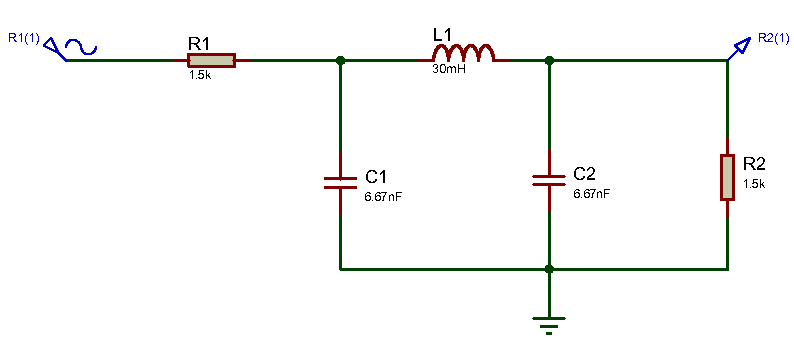
\includegraphics{../Figures/ckt_a}
   \caption{Proteus circuit for low pass filter designed in Problem 1}
   \label{fig:protA}
\end{figure}

\proteusObservationAB{protA}{-6.02}{15.9}{low pass filter designed in Problem 1}

   \begin{figure}[H]
      \centering
      \begin{subfigure}{0.49\textwidth}
         \centering
      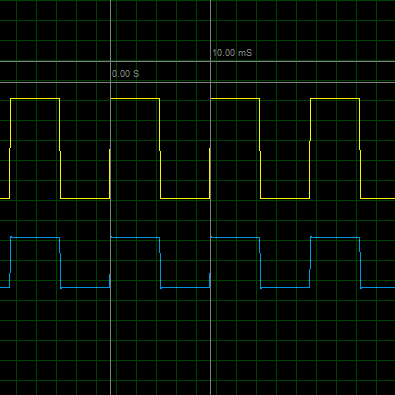
\includegraphics[width=0.9\linewidth]{../Figures/osc_a_1.png}
      \caption{When square wave of 100 Hz is applied}
      \end{subfigure}~
      \begin{subfigure}{0.49\textwidth}
         \centering
         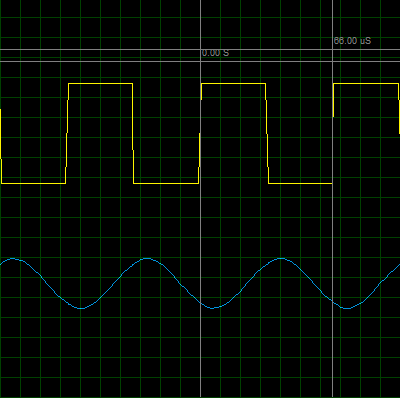
\includegraphics[width=0.9\linewidth]{../Figures/osc_a_2.png}
         \caption{When square wave of 15 KHz is applied}
         \end{subfigure}
         \caption{Observation for application of square wave to circuit shown in Figure \ref{fig:protA}}
      \label{fig:osc_a}
   \end{figure}
   Figure~\ref{fig:osc_a} shows the observation of oscilloscope when a square wave is applied to the designed low pass circuit. For low frequency of 100 Hz, attenuation is visible, but the shape on the output side is still a square wave. This is because the circuit itself is a resistive one, which attenuates the signal. However, when the frequency of the square wave is gradually increased, distortion is visible. For a square wave of frequency about 15 KHz, a sine wave is seen at the output. This is because only some harmonics of the input signal are passed through the filter. 
   

\problem{From the circuit given in Figure \ref{fig:ques}, design a high pass filter having $\omega_0$ of 50000 rad/sec. The
inductance in your final circuit must be of 60 mH. Realize the circuit and plot the magnitude
response. Also show the highest gain in dB and half power frequency in your plot. Observe the output in an oscilloscope when the square wave of 100 Hz is applied at input. Observe the output by increasing frequency up to 10 KHz. Comment on the result.}

Here,
\begin{fleqn}[\parindent]
   \begin{equation*}
      \begin{split}
         &\text{Half power frequency of given normalized filter } (\omega)=1 \text{ rad/s}\\
         &\text{Required half power frequency for high pass filter }(\Omega_0)=50000 \text{ rad/s} 
         \end{split}
      \end{equation*}
\end{fleqn}
While using frequency transformation to design a high pass filter from a normalized low pass filter, the inductor in the original circuit is converted to a capacitor and a capacitor is converted to an inductor. The relation is given in Equation~\ref{eqn:l_hp} and \ref{eqn:c_hp}.
\begin{fleqn}[\parindent]
   \begin{equation*}
      \begin{split}
         &\text{Inductance in given normalized filter } (L_{LP})=2 \text{ H}\\
         &\text{Capacitance in given normalized filter } (C_{LP})=1 \text{ F}\\
         &\text{Mapped capacitance in high pass filter }(C_{HP})=\frac{1}{\Omega_0L_{LP}}=\frac{1}{50000\times2}=1\times10^{-5} \text{ F} \\
         &\text{Mapped inductance in high pass filter }(L_{HP})=\frac{1}{\Omega_0C_{LP}}=\frac{1}{50000\times1}=2\times10^{-5}\text{ H} 
         \end{split}
      \end{equation*}
\end{fleqn}
According to the problem, we have a restriction on the value of the inductor such that the inductance in the final circuit must be 60 mH. Since the obtained values are for high pass at the required frequency, only magnitude scaling is performed to get the values as required. So, we back-calculate the value of magnitude scaling factor $(K_m)$ using Equation~\ref{eqn:l_mag}.

\begin{fleqn}[\parindent]
   \begin{equation*}
      \begin{split}
         &\text{Required value of inductance } (L_{new})=60 \text{ mH}\\
         &\text{Old value of inductance }(L_{old})=L_{HP}=2\times10^{-5} \text{ H} 
      \end{split}
      \end{equation*}
\end{fleqn}
\begin{fleqn}[\parindent]
   \begin{equation*}
      \begin{split}
         &L_{new}=K_m.L_{old}\\
         &\Rightarrow K_m = \frac{L_{new}}{L_{old}} = \frac{60\times10^{-3}}{2\times10^{-5}}=3000
      \end{split}
      \end{equation*}
\end{fleqn}
From this scaling factor we can calculate the new values of the resistor and capacitor from $R_{old}=1\Omega$ and $C_{old}=1\times10^{-5}$ F using Equation~\ref{eqn:r_mag} and \ref{eqn:c_mag},
\begin{fleqn}[\parindent]
   \begin{equation*}
      \begin{split}
         &R_{new}=K_m.R_{old}=3000\times1=3000 \text{ }\Omega=3\text{ K}\Omega\\
         &C_{new}=\frac{C_{old}}{K_m}=\frac{1\times10^{-5}}{3000}=3.33 \text{ nF}
      \end{split}
      \end{equation*}
\end{fleqn}

\begin{figure}[H]
   \centering
   \figb
   \caption{Final circuit for high pass filter designed in Problem 2}
   \label{fig:figb}
\end{figure}

\begin{figure}[H]
   \centering
   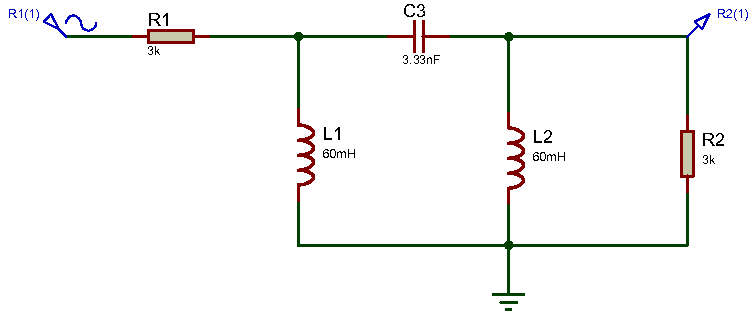
\includegraphics{../Figures/ckt_b}
   \caption{Proteus circuit for high pass filter designed in Problem 2}
   \label{fig:protB}
\end{figure}

\proteusObservationAB{protB}{-6.02}{7.95}{high pass filter designed in Problem 2}


   \begin{figure}[H]
      \centering
      \begin{subfigure}{0.49\textwidth}
         \centering
      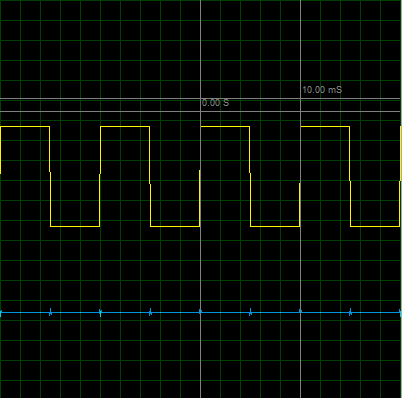
\includegraphics[width=0.9\linewidth]{../Figures/osc_b_1.png}
      \caption{When square wave of 100 Hz is applied}
      \end{subfigure}~
      \begin{subfigure}{0.49\textwidth}
         \centering
         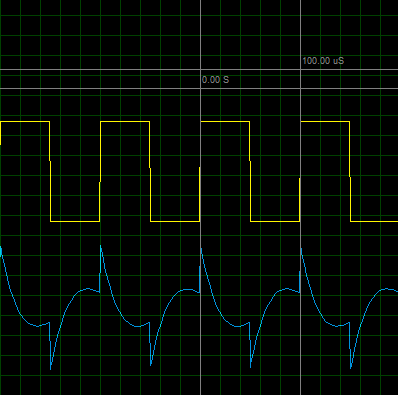
\includegraphics[width=0.9\linewidth]{../Figures/osc_b_2.png}
         \caption{When square wave of 10 KHz is applied}
         \end{subfigure}
         \caption{Observation for application of square wave to circuit shown in Figure \ref{fig:protB}}
      \label{fig:osc_b}
   \end{figure}

   Figure~\ref{fig:osc_b} shows the observation of oscilloscope when a square wave is applied to the designed high pass circuit. Unlike the low pass circuit, the high pass filter doesn't show some fixed wave behavior. For low frequency signal, output is essentially a flat line except for some spikes representing the higher frequency components. Whereas when the frequency is increased, spikes appear on the output. This is due to the high frequency transition of the signal.
   

\problem{From the circuit given in Figure \ref{fig:ques}, design a band pass filter having $\omega_0$ of 40000 rad/sec and
Bandwidth of 4000 rad/sec. In your final design the largest inductance should be of 1H and all
other elements should be practically realizable. Realize the circuit and plot the magnitude
response. Also show the highest gain in dB, gain at 40000 rad/sec and half power frequencies in
your plot.}


Here,
\begin{fleqn}[\parindent]
   \begin{equation*}
      \begin{split}
         &\text{Half power frequency of given normalized filter } (\omega)=1 \text{ rad/s}\\
         &\text{Required center frequency for band pass filter }(\Omega_0)=40000 \text{ rad/s} \\
         &\text{Required bandwidth for band pass filter }(B)=4000 \text{ rad/s} 
         \end{split}
      \end{equation*}
\end{fleqn}
While using frequency transformation to design a band pass filter from a normalized low pass filter, the inductor in the original circuit is converted to a series LC combination and a capacitor is converted to a parallel LC combination. The relation is given in Equation~\ref{eqn:l_bp} and \ref{eqn:c_bp}.
\begin{fleqn}[\parindent]
   \begin{equation*}
      \begin{split}
         &\text{Inductance in given normalized filter } (L_{LP})=2 \text{ H}\\
         &\text{Capacitance in given normalized filter } (C_{LP})=1 \text{ F}\\
         &\text{For mapped elements in band pass filter arising due to inductance in normalized filter:}\\
         &\text{Series inductance }(L_{BP}^s)=\frac{L_{LP}}{B}=\frac{2}{4000}=5\times10^{-4} \text{ H}\\
         &\text{Series capacitance }(C_{BP}^s)=\frac{B}{\Omega_0L_{LP}}=\frac{4000}{(40000)^2\times2}=1.25\times10^{-6}\text{ F}\\
         &\text{For mapped elements in band pass filter arising due to capacitance in normalized filter:}\\
         &\text{Parallel inductance }(L_{BP}^p)=\frac{B}{\Omega^2C_{LP}}=\frac{4000}{(40000)^2\times1}=2.5\times10^{-6} \text{ H}\\
         &\text{Parallel capacitance }(C_{BP}^p)=\frac{C_{LP}}{B}=\frac{1}{4000}=2.5\times10^{-4} \text{ F}
         \end{split}
      \end{equation*}
\end{fleqn}

According to the problem, we have a restriction on the value of the inductor such that the largest inductance in the final circuit must be 1 H. Since the obtained values are for band pass at the required frequency and bandwidth, only magnitude scaling is performed to get the values as required. So, we back-calculate the value of magnitude scaling factor $(K_m)$ using Equation~\ref{eqn:l_mag}.

\begin{fleqn}[\parindent]
   \begin{equation*}
      \begin{split}
         &\text{Required value of inductance } (L_{new})=1 \text{ H}\\
         &\text{Old value of inductance }(L_{old})=L_{BP}^s=5\times10^{-4} \text{ H} 
      \end{split}
      \end{equation*}
\end{fleqn}
\begin{fleqn}[\parindent]
   \begin{equation*}
      \begin{split}
         &L_{new}=K_m.L_{old}\\
         &\Rightarrow K_m = \frac{L_{new}}{L_{old}} = \frac{1}{5\times10^{-4}}=2000
      \end{split}
      \end{equation*}
\end{fleqn}

From this scaling factor we can calculate the new values of the resistor, inductor and capacitor from $R_{old}=1\Omega$, $L_{old}^p=2.5\times10^{-6}$ H, $C_{old}^s=1.25\times10^{-6}$ F and $C_{old}^p=2.5\times10^{-4}$ F using Equation~\ref{eqn:r_mag} and \ref{eqn:c_mag},
\begin{fleqn}[\parindent]
   \begin{equation*}
      \begin{split}
         &R_{new}=K_m.R_{old}=2000\times1=2000 \text{ }\Omega=2\text{ K}\Omega\\
         &L_{new}^p=K_m.L_{old}^p=2000\times2.5\times10^{-6}=5\times10^{-3} \text{ H}=5\text{ mH}\\
         &C_{new}^s=\frac{C_{old}^s}{K_m}=\frac{1.25\times10^{-6}}{2000}=0.625 \text{ nF}\\
         &C_{new}^p=\frac{C_{old}^p}{K_m}=\frac{2.5\times10^{-4}}{2000}=0.125 \text{ }\mu \text{F}
      \end{split}
      \end{equation*}
\end{fleqn}

\begin{figure}[H]
   \centering
   \figc
   \caption{Final circuit for band pass filter designed in Problem 3}
   \label{fig:figc}
\end{figure}


\begin{figure}[H]
   \centering
   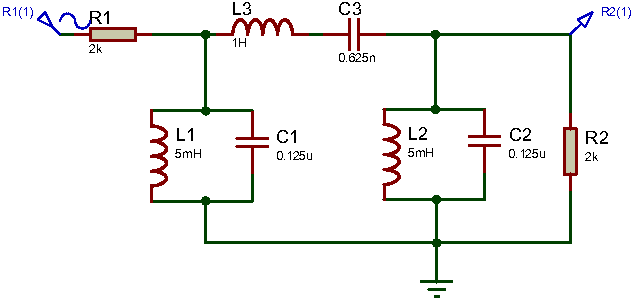
\includegraphics{../Figures/ckt_c}
   \caption{Proteus circuit for band pass filter designed in Problem 3}
   \label{fig:protC}
\end{figure}

\proteusObservationCD{protC}{-6.02}{6.215, 6.435}{-7.37}{band pass filter designed in Problem 3}


\problem{From the circuit given in Figure \ref{fig:ques}, design a band stop filter having $\omega_0$ of 40000 rad/sec and Bandwidth of 4000 rad/sec. In your final design the largest inductance should be of 1H and all other elements should be practically realizable. Realize the circuit and plot the magnitude response. Also show the highest gain in dB, gain at 40000 rad/sec and half power frequencies in your plot.}
\pagebreak
Here,
\begin{fleqn}[\parindent]
   \begin{equation*}
      \begin{split}
         &\text{Half power frequency of given normalized filter } (\omega)=1 \text{ rad/s}\\
         &\text{Required center frequency for band stop filter }(\Omega_0)=40000 \text{ rad/s} \\
         &\text{Required bandwidth for band stop filter }(B)=4000 \text{ rad/s}
         \end{split}
      \end{equation*}
\end{fleqn}
While using frequency transformation to design a band stop filter from a normalized low pass filter, the inductor in the original circuit is converted to a parallel LC combination and a capacitor is converted to a series LC combination. The relation is given in Equation~\ref{eqn:l_bs} and \ref{eqn:c_bs}.
\begin{fleqn}[\parindent]
   \begin{equation*}
      \begin{split}
         &\text{Inductance in given normalized filter } (L_{LP})=2 \text{ H}\\
         &\text{Capacitance in given normalized filter } (C_{LP})=1 \text{ F}\\
         &\text{For mapped elements in band stop filter arising due to inductance in normalized filter:}\\
         &\text{Parallel inductance }(L_{BS}^p)=\frac{BL_{LP}}{{\Omega_0}^2}=\frac{4000\times2}{40000^2}=5\times10^{-6}\text{ H}\\
         &\text{Parallel capacitance }(C_{BS}^p)=\frac{1}{BL_{LP}}=\frac{1}{4000\times2}=1.25\times10^{-4}\text{ F}\\
         &\text{For mapped elements in band stop filter arising due to capacitance in normalized filter:}\\
         &\text{Series inductance }(L_{BS}^s)=\frac{1}{BC_{LP}}=\frac{1}{4000\times1}=2.5\times10^{-4}\text{ H}\\
         &\text{Series capacitance }(C_{BS}^s)=\frac{BC_{LP}}{{\Omega_0}^2}=\frac{4000\times1}{40000^2}=2.5\times10^{-6}\text{ F}\\
         \end{split}
      \end{equation*}
\end{fleqn}

According to the problem, we have a restriction on the value of the inductor such that the largest inductance in the final circuit must be 1 H. Since the obtained values are for band stop at the required frequency and bandwidth, only magnitude scaling is performed to get the values as required. So, we back-calculate the value of magnitude scaling factor $(K_m)$ using Equation~\ref{eqn:l_mag}.

\begin{fleqn}[\parindent]
   \begin{equation*}
      \begin{split}
         &\text{Required value of inductance } (L_{new})=1 \text{ H}\\
         &\text{Old value of inductance }(L_{old})=L_{BS}^s=2.5\times10^{-4} \text{ H} \\
      \end{split}
      \end{equation*}
\end{fleqn}
\begin{fleqn}[\parindent]
   \begin{equation*}
      \begin{split}
         &L_{new}=K_m.L_{old}\\
         &\Rightarrow K_m = \frac{L_{new}}{L_{old}} = \frac{1}{2.5\times10^{-4}}=4000\\
      \end{split}
      \end{equation*}
\end{fleqn}

From this scaling factor we can calculate the new values of the resistor, inductor and capacitor from $R_{old}=1\Omega$, $L_{old}^p=5\times10^{-6}$ H, $C_{old}^s=2.5\times10^{-6}$ F and $C_{old}^p=1.25\times10^{-4}$ F using Equation~\ref{eqn:r_mag} and \ref{eqn:c_mag},
\begin{fleqn}[\parindent]
   \begin{equation*}
      \begin{split}
         &R_{new}=K_m.R_{old}=4000\times1=4000 \text{ }\Omega=4\text{ K}\Omega\\
         &L_{new}^p=K_m.L_{old}^p=4000\times5\times10^{-6}=5\times10^{-3} \text{ H}=20\text{ mH}\\
         &C_{new}^s=\frac{C_{old}^s}{K_m}=\frac{2.5\times10^{-6}}{4000}=0.625 \text{ nF}\\
         &C_{new}^p=\frac{C_{old}^p}{K_m}=\frac{1.25\times10^{-4}}{4000}=31.25 \text{ nF}\\
      \end{split}
      \end{equation*}
\end{fleqn}

\begin{figure}[H]
   \centering
   \figd
   \caption{Final circuit for band stop filter designed in Problem 4}
   \label{fig:figd}
\end{figure}


\begin{figure}[H]
   \centering
   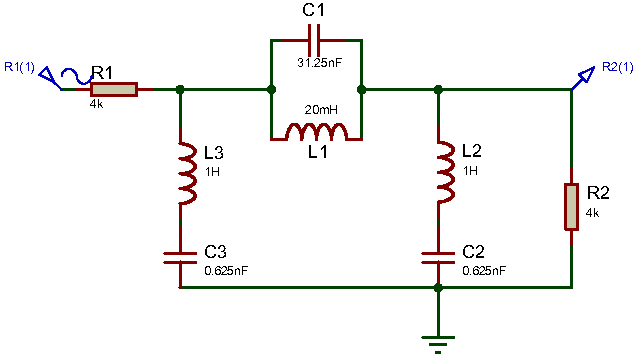
\includegraphics[scale=0.9]{../Figures/ckt_d}
   \caption{Proteus circuit for band pass filter designed in Problem 4}
   \label{fig:protD}
\end{figure}
\proteusObservationCD{protD}{-6.02}{5.1, 7.83}{-49.3}{band stop filter designed in Problem 4}

\section{Discussion and Conclusion}
In this lab experiment, we learnt about impedance scaling, frequency scaling and frequency transformation. Although these topics are dealt in our regular course content, hands on designing of different types of filters such as low pass at required half power frequency, high pass at required half power frequency, band pass and band stop filters with required center frequency and bandwidth from normalized prototype filter allowed better understanding of the topics. Impedance scaling is used to map components to practically realizable values, which are generally limited during actual design. Frequency scaling is used to shift filter response on the frequency axis. Frequency transform is used to convert said normalized filter into high pass, band pass or band stop filter using the derived equations.\\The exercises in Problem 1 and Problem 2 were fairly straight forward with the use of impedance and frequency scaling and frequency transformation. However, for Problem 3 and Problem 4, although the mapped components are theoretically correct, Proteus simulation, workbench simulation gave unexpected results with the half power frequency and gain at center frequency. The reason behind such behavior is unknown, since the values are mapped correctly. Frequency plot using other online simulation tool seem correct, but the same circuit has shown quite peculiar behavior.\\
Hence, the objectives of the lab were fulfilled with the understanding of the necessity of the mentioned topics. However, the issue seen with the response is yet to be figured out.
\end{document}